%
% Prototype Formation
%

\section{Category Learning in Autism}
%We have shown how the overly perseverative top-down attentional influence of the PFC could underlie an extensive array of behaviors in people with ASD.  In this last chapter before concluding and summarizing my work, we investigate if differences in concept formation in people with ASD can be included in the list of behaviors encompassed by my theory.  

Prototype formation is an important skill and is believed to be invaluable in learning to categorize information in our environment.  The prototype for a specific category is a representational average of all the features of examples previously seen for that category.  The ability to learn an abstract representation of a category can greatly reduce the memory demands on an individual. Recent studies suggest when learning a new concept or category, children with autism are less likely to form and use a prototype representation when compared to normally developing individuals~\cite{RefWorks:113,StraussMS:2009:Prototype}.  Difficulty in forming and properly using an abstracted prototype is argued by some researchers to underly many of the generalization problems found in people with ASD.   Both of the aforementioned studies investigated the ability to form a prototype via a phenomena known as the ``prototype effect''.  The ``prototype effect'' is a phenomena in which the prototype is preferably remembered as a member of the category when compared to other possible examples, even though it was not experienced previously.  The results of these studies suggest that people with ASD do not demonstrate the ``prototype effect'' during a standard category learning task.  Our modeling efforts will concentrate on the study by Klinger and Dawson (2001), which we describe next. 

\subsection{Investigating Prototype Formation}
In order to investigate prototype formation in people with ASD,  Klinger and Dawson (2001) had subjects perform a basic categorization task.  There were two phases to the experiment.  The first phase was a familiarization task in which subjects were exposed to a variety of examples of imaginary animals.  This phase was used to teach the subjects a single animal category. (See Figure~\ref{prototype-categories}.) The second phase was a testing phase requiring the subjects to identify the animal which was the best example of the imaginary category that they had learned.   Each imaginary animal belonged to a specific category, and members of each category possessed four category-specific features of interest, each of which could have a range of different discrete values.  For instance, an item belonging to the ``Mip'' category would display horns, wings, mouths, and feet, with different Mips having different horn widths, wing widths, mouth widths, and foot lengths.  Each feature ranged in five discrete steps from smallest to largest values.  For example, the horn widths smallest value could be 2.5 cm and each subsequent length increasing by a constant .50 cm resulting in five discrete lengths ranging from 2.5 cm to 4.5 cm.  The smallest length for each feature was labeled with a value of 1, the second longest was labeled with a value of 2, up to the largest length which was labeled with a value of 5 for coding purposes.  This coding scheme allows for the four digit encoding of individual stimuli, with the different numbers representing the respective values of the features they represent (e.g. ``5115'' where each number corresponds to a value of a distinct feature of the imaginary animal). 

During the familiarization phase subjects were shown eight examples of a category compared to eight non-member examples (e.g. Mip vs. Pev;  Mip vs. Dak; etc.).  On the first familiarization trial, subjects were given the name of the target category (e.g. ``This is a Mip''), and asked to identify the target in all subsequent trials.  Target categories were able to be identified by simply noting the presence of features specific to each respective category.  Specifically, it was not necessary to attend to the different feature values for correct categorization.  For instance, an instance of the ``Mip'' category has horns and an octangular body, no other imaginary animal category possessed these features.  Feedback was provided on each trial, providing praise if the correct category was selected, and correcting the response otherwise.  Familiarization stimuli were constructed such that the children would see target category examples that contained feature values 1, 2, 4, and 5, but never 3. (See Figure~\ref{mip-familiarization}.)  After all familiarization trials, the average value used for each feature in the target category was 3, resulting in an average prototype for the category possessing the feature values of 3333 (all average lengths and widths of the possible four features in the target category).  

Testing immediately followed the familiarization phase.  During testing, a prototypical example for the category (3333) was paired with a previously seen familiarization example (e.g. 5511) or a novel stimulus comprised of previously experienced feature values (e.g. 1551).  Subjects were asked to select which example was the ``best'' category member.  Normally developing individuals choose the prototype at a rate significantly higher than chance.  However, people with autism selected the prototype exemplar at chance levels when comparing to non-prototype stimuli (e.g. the novel or familiar stimuli). (See Figure~\ref{klinger_results}.)  The authors argued that this effect demonstrates a lack of prototype abstraction in people with autism.  

\begin{figure}[ht]
\begin{center}
	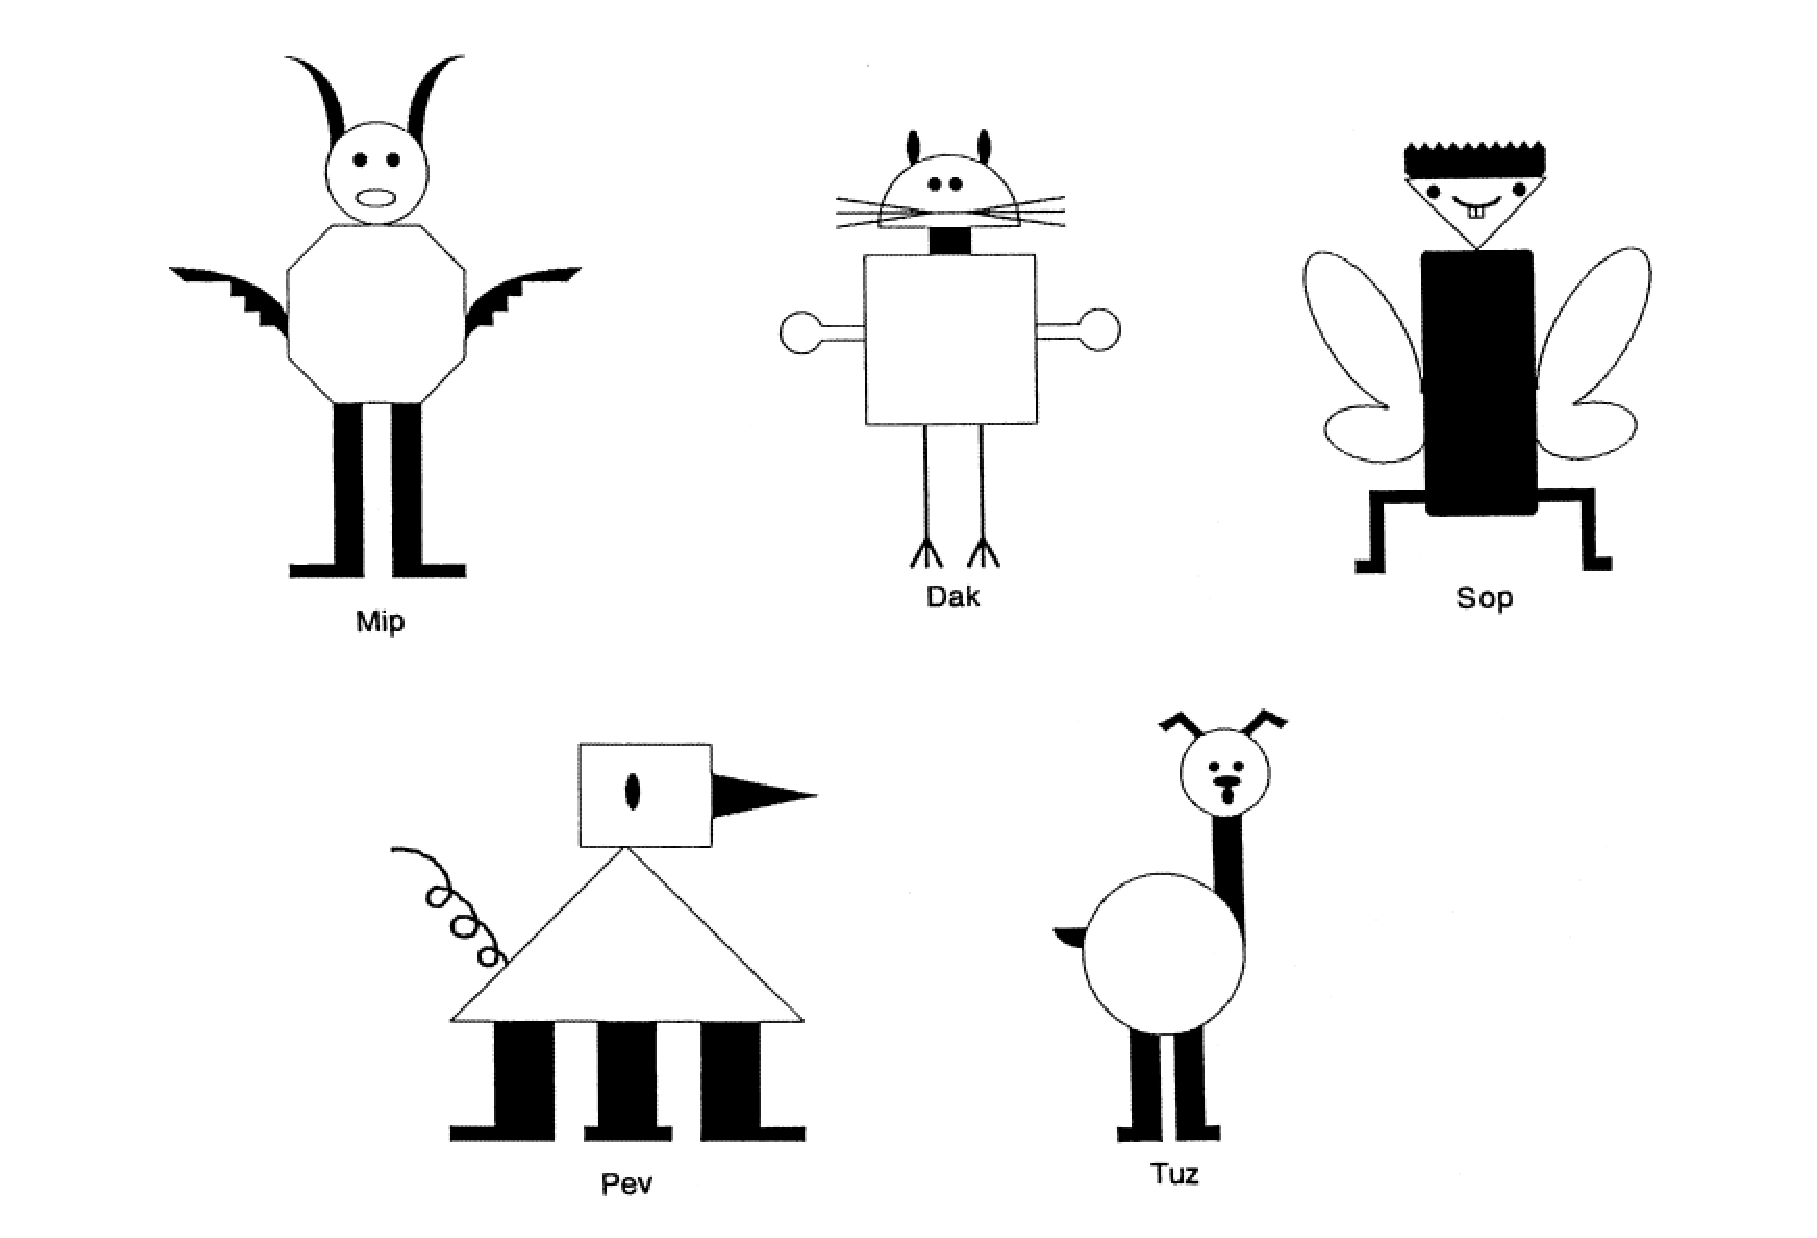
\includegraphics[width=100mm]{figures/prototype_categories.eps}
\end{center}
\caption{Examples of different members of a category used in the prototype learning experiment.  Image adapted from (Klinger and Dawson, 2001).}
\label{prototype-categories}
\end{figure} 

\begin{figure}[ht]
\begin{center}
	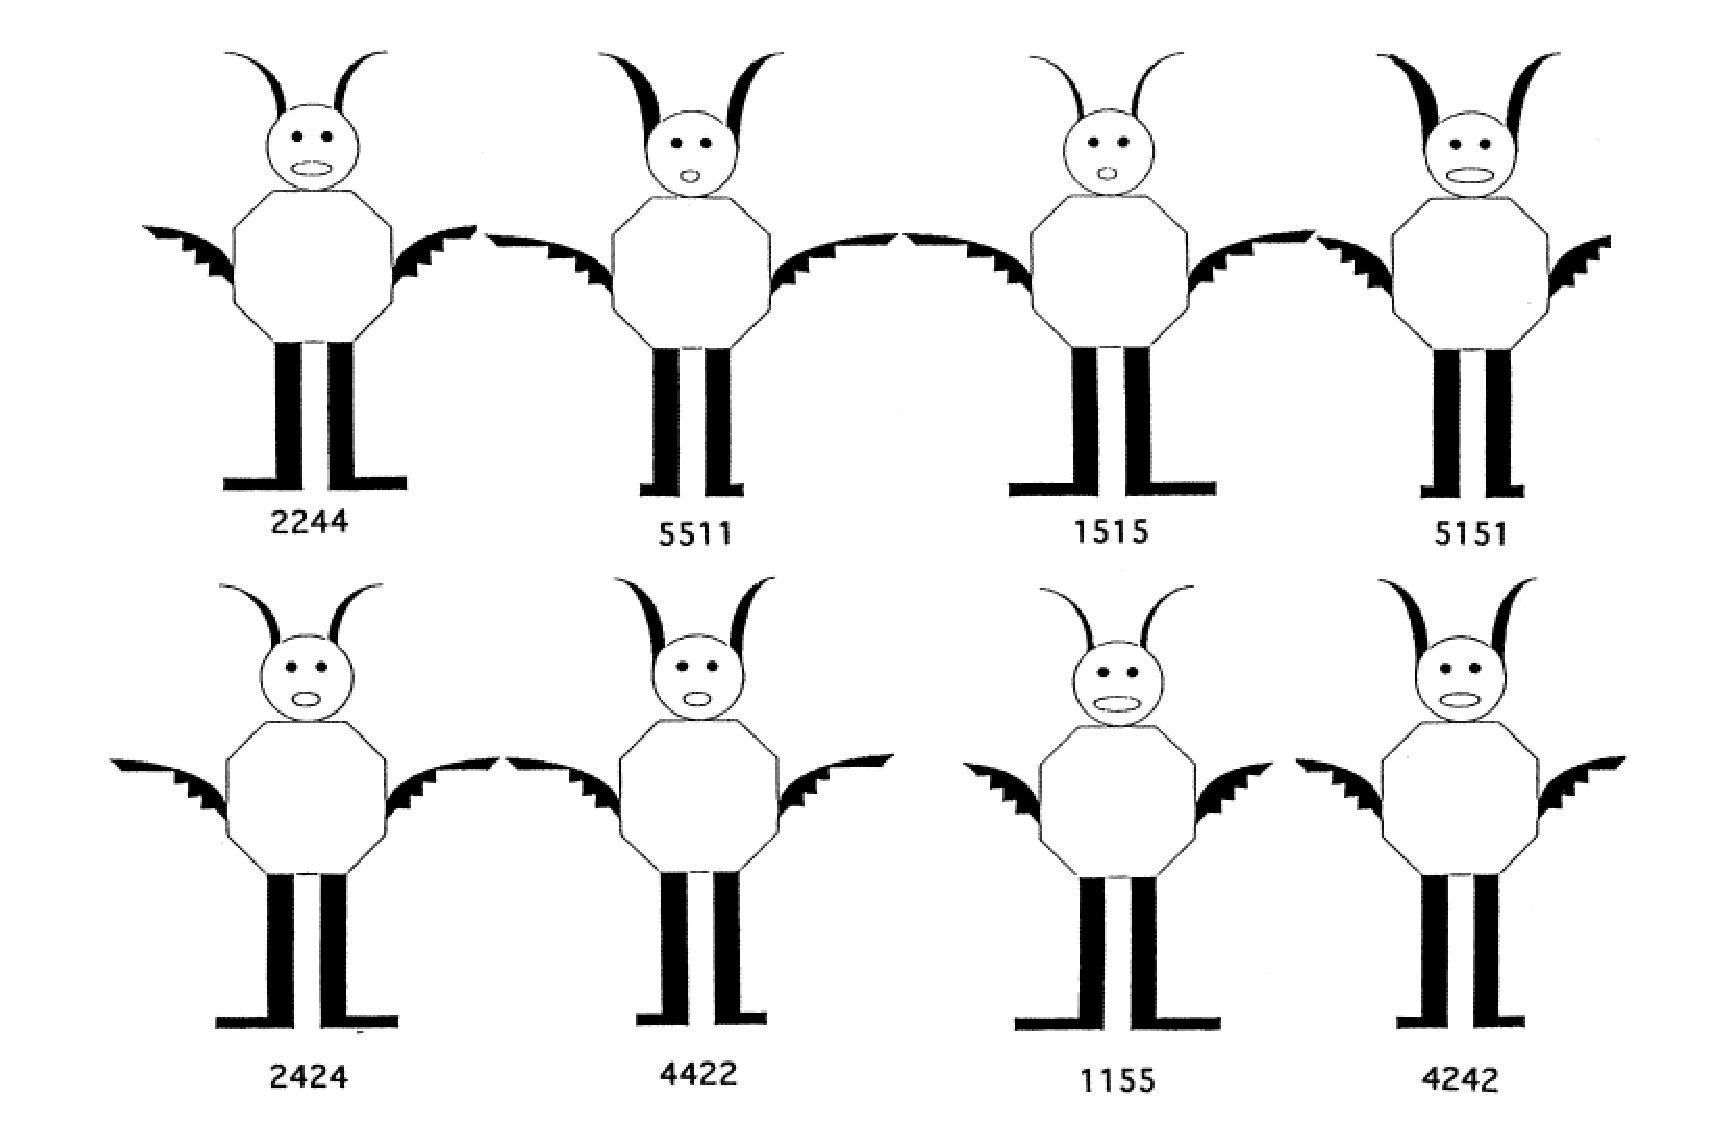
\includegraphics[width=100mm]{figures/mip_familiarization.eps}
\end{center}
\caption{Examples of different categories used in the prototype learning experiment.  Image adapted from (Klinger and Dawson, 2001).}
\label{mip-familiarization}
\end{figure} 

\begin{figure}[ht]
\begin{center}
	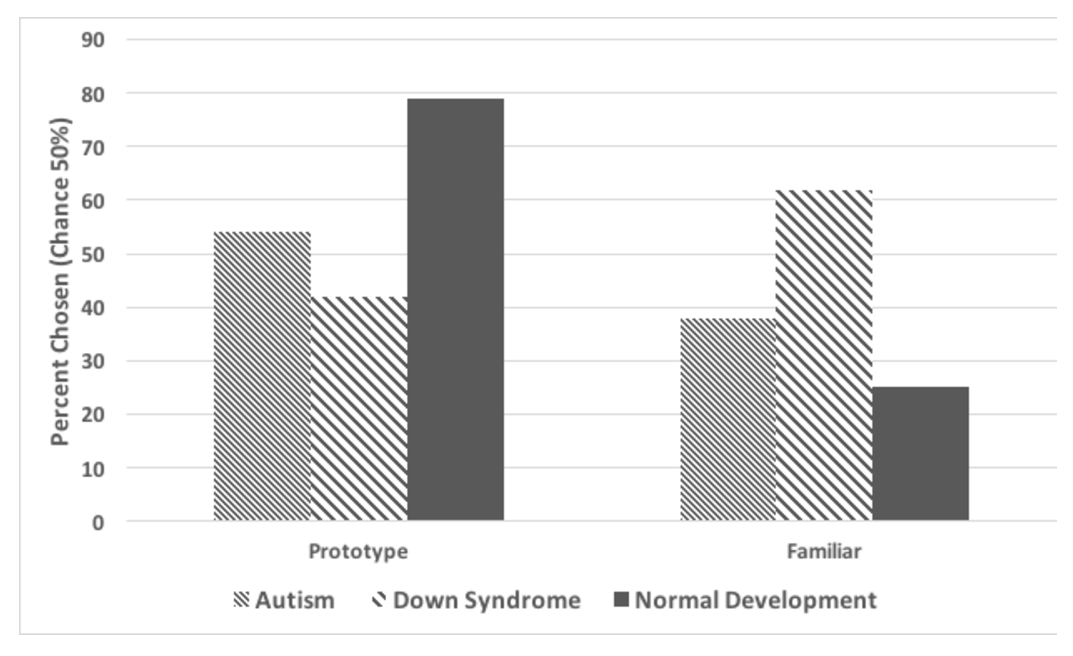
\includegraphics[width=110mm]{figures/klinger_results.eps}
\end{center}
\caption{Results adapted from (Klinger and Dawson, 2001).  The measure on the y-axis is the percentage of times that the prototypical animal was chosen over either a novel or familiar example. Their results indicate that the normally developing group chose the prototype at greater than chance levels, clearly demonstrating a prototype effect.  However, the ASD group did not show a prototype effect, this is argued to support the authors conjecture that people with ASD do not form or utilize prototype representations in categorization tasks. (Please note: Only the ``Prototype'' condition is relevant to the discussion.  The results for ``Familiar'' refer to a comparison in the original study investigating if there was a preference for previously experienced or novel animals.)}
\label{klinger_results}
\end{figure} 

\subsection{Modeling Category Learning with ALCOVE}
ALCOVE is a formal computational model of human performance in category learning~\cite{RefWorks:114} and has been highly successful at capturing human category learning performance when classification feedback on example category members is provided.  ALCOVE will learn, after repeated exposure to examples and explicit feedback, what stimulus dimensions are important for correct categorization of the examples.  There are three main processing layers used in ALCOVE, an input layer with units representing stimulus features in psychological space.  The hidden layer contains units that roughly represent the ``location'' of stimuli in psychological space.  The activation profile of the hidden layer is similar to an exponentially decaying radial basis function, the closer in psychological space an input vector presented to ALCOVE is to the ``location'' of a hidden layer unit, the higher the activation level of the unit.  The level of hidden unit activation decays in an exponential fashion as a function of the distance between the location of the hidden unit and the input to the network.  The output units are standard linear units summing the activation across weighted connections from the hidden layer units.  It is useful to view these units as representing different category labels (e.g. ``Mip''). In order to match human performance, the activation levels of the output units are scaled to response probabilities using a Luce Choice Rule:

\begin{equation}
P(B) = exp(\phi a_B) / \sum (exp(\phi a_b))
\label{luce-choice}
\end{equation}\\
$P(B)$ computes the probability of selecting the category $B$ for a stimulus being presented to the network, $a_B$ is the activation level of the output unit representing category $B$, $\sum (exp(\phi a_b))$ is the sum over the exponential value of all of the output activations, and  $\phi$ is a gain parameter used to scale the results.

Importantly, for our purposes, ALCOVE utilizes a set of dimensional attention ``weights'', or parameters, when learning to categorize stimulus objects.  These parameters are constrained to the range between 0 and 1, and, conceptually, as the parameter value increases the more sensitive the model is to changes along this feature dimension.  ALCOVE's dimensional attention weights capture the degree to which attention should be spread over stimulus features and, thus, are analogous to the hypothesized role of PFC in directing top-down attentional control.  In the ALCOVE framework, perseverative attention would limit dimensional attention weights, resulting in an overweighting of a small number of the available features.  As described below, limiting ALCOVE's dimensional attention weights in this way allows us to capture the performance of individuals with autism as documented by Klinger and Dawson (2001). 

\begin{figure}[ht]
\begin{center}
	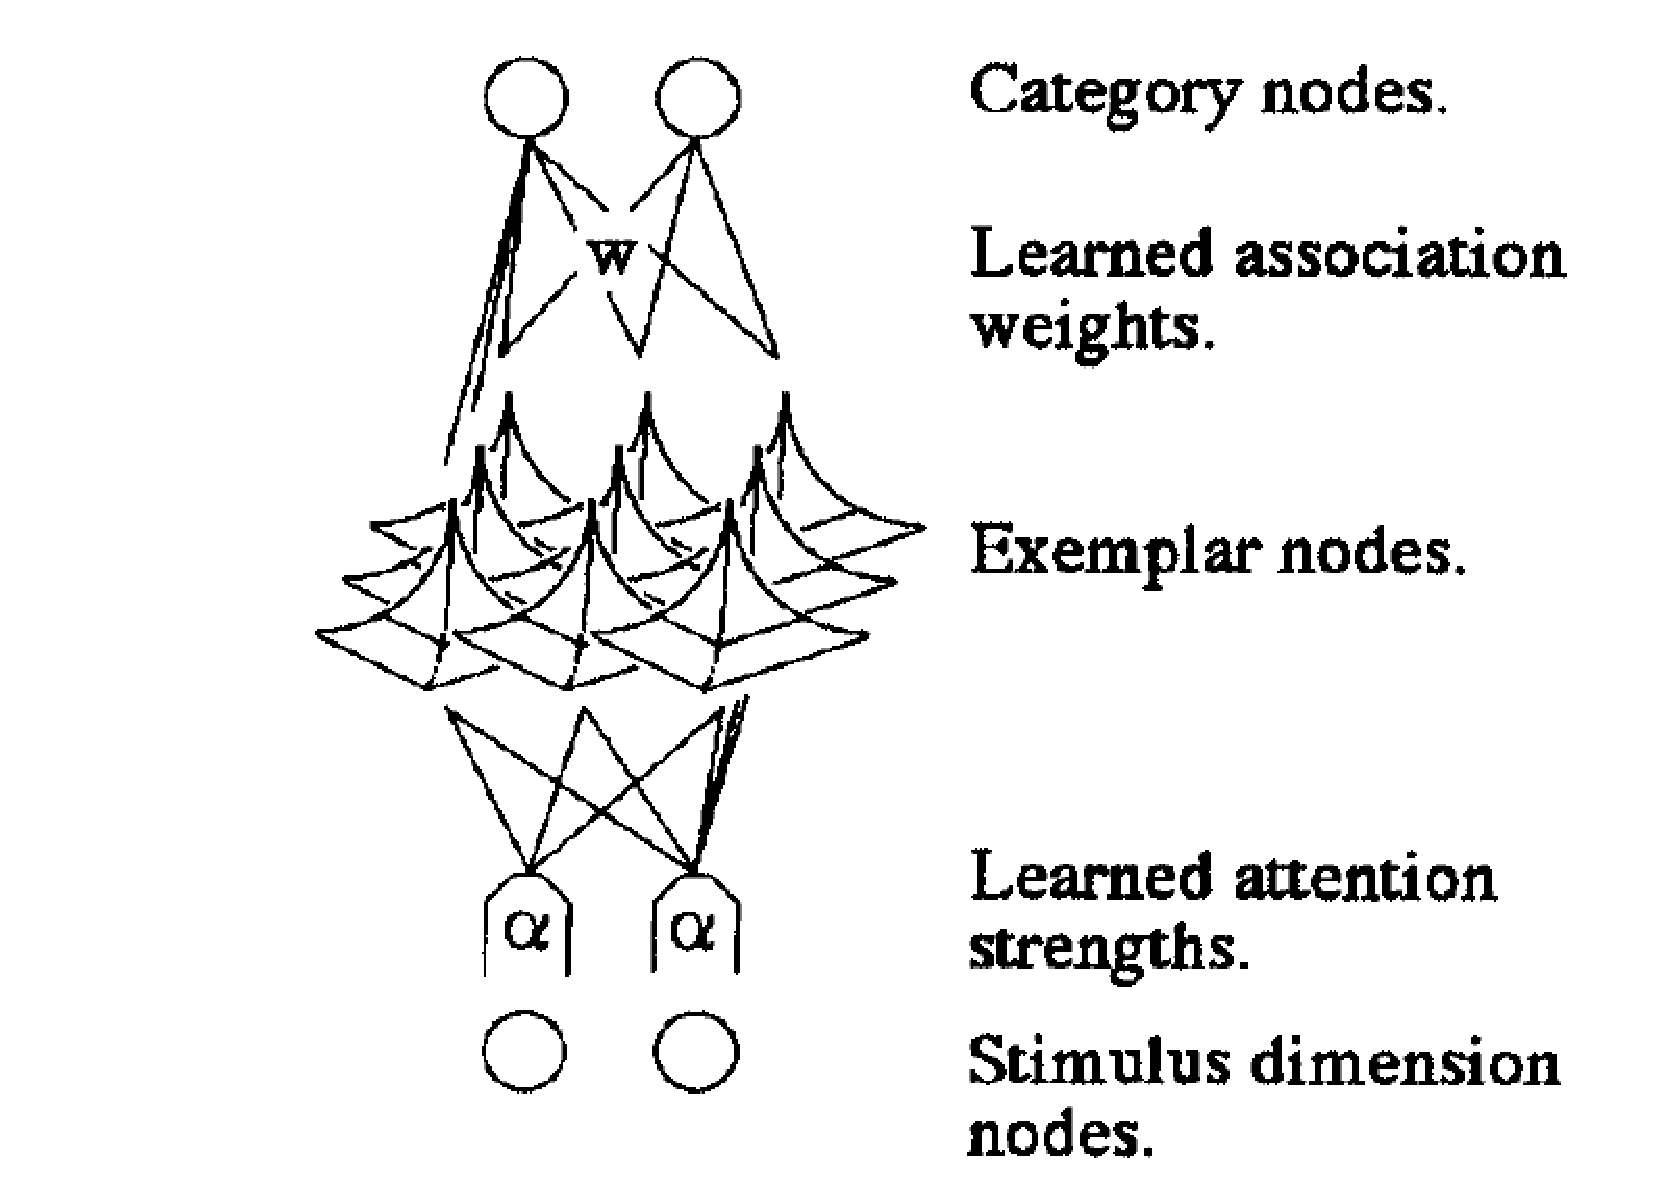
\includegraphics[width=100mm]{figures/alcove.eps}
\end{center}
\caption{Structure of ALCOVE (Attention Learning CoVEring map).  Image adapted from (Kruschke, 1992).}
\label{alcove}
\end{figure} 

\subsection{Prototype Learning in ALCOVE}
The training and testing of ALCOVE was modeled after the Klinger et al. study described above.  The training corpus was based on examples identical, in principal, to the target categories used during the familiarization trials. (See Figure~\ref{mip-familiarization}.)  As in the original study, eight familiarization trials were presented to the network during training.  On each presentation, the model was required to label each target stimulus (e.g. this is a ``Mip'').  Only two response units (``Mip'' \& ``Non-Mip''), were required in order for the network to perform the task.  Four input units, each with dimensional attention weights, were activated for each example presented to the network.  The four input units represent the four unique varying features used within each category in the behavioral study.  The level of activation for each input varied in a systematic fashion in accordance with the feature value of the stimulus.  For instance, if the stimuli presented has feature values (1551), the input vector presented to the network used the values (.20 1.0 1.0 .20). The same eight familiarization stimuli as were used in the Klinger et al. study were presented to the ALCOVE network, simulating the same learning environment as the subjects experienced.  The standard ALCOVE error correction weight adjustments were used during the entirety of training.   After training ALCOVE on the familiarization stimuli, testing proceeded with all learning disabled in the model.  

During testing, the prototype (3333) and the non-prototype test items, a novel stimuli (e.g. 1551) and a previously seen familiarization stimuli (e.g. 1515), were presented to ALCOVE separately.  The overall activation level of the output unit for the target category was recorded and used to determine which stimuli type was the ``preferred'' category example for ALCOVE.  In other words, the higher the activation of the output unit corresponding to the correct category, the stronger the ``vote'' for the example presented to the network.  The model always correctly categorized each stimuli regardless if it was a prototype, novel, or previously seen example. In order to compare model preference between prototype and non-prototype stimuli the activation levels were scaled to response probabilities using a Luce Choice Rule. (See Equation~\ref{luce-choice}.).  The average response probability for prototype versus non-prototype stimuli is the measure used in the comparison to the actual experiment results. 

\subsection{Modeling Autism in ALCOVE}
In order to simulate autistic performance we artificially biased one randomly selected attentional dimension by strengthening the weighting of that dimension's attentional weight in ALCOVE.  This was done by simply hand coding one of the attentional weights at an extremely high value (.9).  The other dimensional attention weights were all initialized to low values (.1).  This manipulation captures, at a gross level, my conjecture that deficient dopamine based gating of PFC representations will result in overly perseverative attention to a restricted set of features or dimensions.  In the control version of the model, the dimensional attention weights were spread out evenly and all initially set to a low level (.1), as is standard in ALCOVE, allowing the network to allocate its attention in a more appropriate manner.  These parameters were adjusted by the standard ALCOVE learning rule for dimensional attention weights throughout the training process in both the control and autistic-like conditions.  One additional ALCOVE parameter was adjusted in order to better simulate the performance of people with autism on the categorization task.  The standard ALCOVE equation for the activation levels of the exponentially decaying hidden units contains a multiplicative scaling parameter referred to  by Kruschke as ``specificity''.  As this parameter increases, the activation profile of the hidden unit becomes more narrow, resulting in a smaller range of feature values that are capable of highly activating the unit.  In other words, increasing the specificity parameter makes the hidden units in ALCOVE hyper-specific, sensitive to a more-restrictive range of features in the environment.  This is interesting because many researchers have argued that people with autism exhibit hyper-specific behavior in their everyday lives~~\cite{McClellandJL:2000:Autism,HappeF:1999:WCC}.  In the results described next, the specificity parameter in ALCOVE was adjusted from 1.0 in the control network to 2.5 for the network modeling behavior of people with ASD.  The manipulation of the specificity parameter in ALCOVE has been previously used and justified to capture performance of a clinical population during the investigation of categorization behavior in amnesic patients~\cite{NosofskyRM:1998:LCOVEAmnesia}. 

%The simulated performance of people with autism will be contrasted with the control case, believed to capture normally developing people's performance on such tasks.  The performance of both autistic and control ALCOVE models will be directly compared to the data collected by Klinger and Dawson (2001). 

\subsection{Prototype Formation Simulation Results}

Network simulations were repeated 80 times in each of the experimental conditions, with each repetition treated as an individual subject for data analysis.  The control network was able to reproduce the prototype effect as observed in normally developing individuals, choosing the prototype over the non-prototype 70.52\% of the time.  (See Figure~\ref{alcove-results}.)  For consistency we used to the same analysis as Klinger et al. (2001), a one-sample T-test, in order to determine if the model's preference for the prototype over non-prototype stimuli was statistically reliably different from chance (50\%).  The analysis of the control model's performance indicated that the prototype effect was indeed significantly different, and larger, than chance (T-Value: 4.05; $p < .0001$).   Looking at the performance of the model of autistic behavior, however, we see a very different profile. (See Figure~\ref{alcove-results}.)  The ASD network preferred the prototype over the non-prototype stimuli only 52.91\% of the time according to our measure, and statistical analysis confirms that this is not significantly larger than chance (T-Value: 0.52; $p > .30$).  This matches the lack of a prototype effect in people with autism found in previous behavioral studies~\cite{RefWorks:113,StraussMS:2009:Prototype}.

\begin{figure}[ht]
\begin{center}
	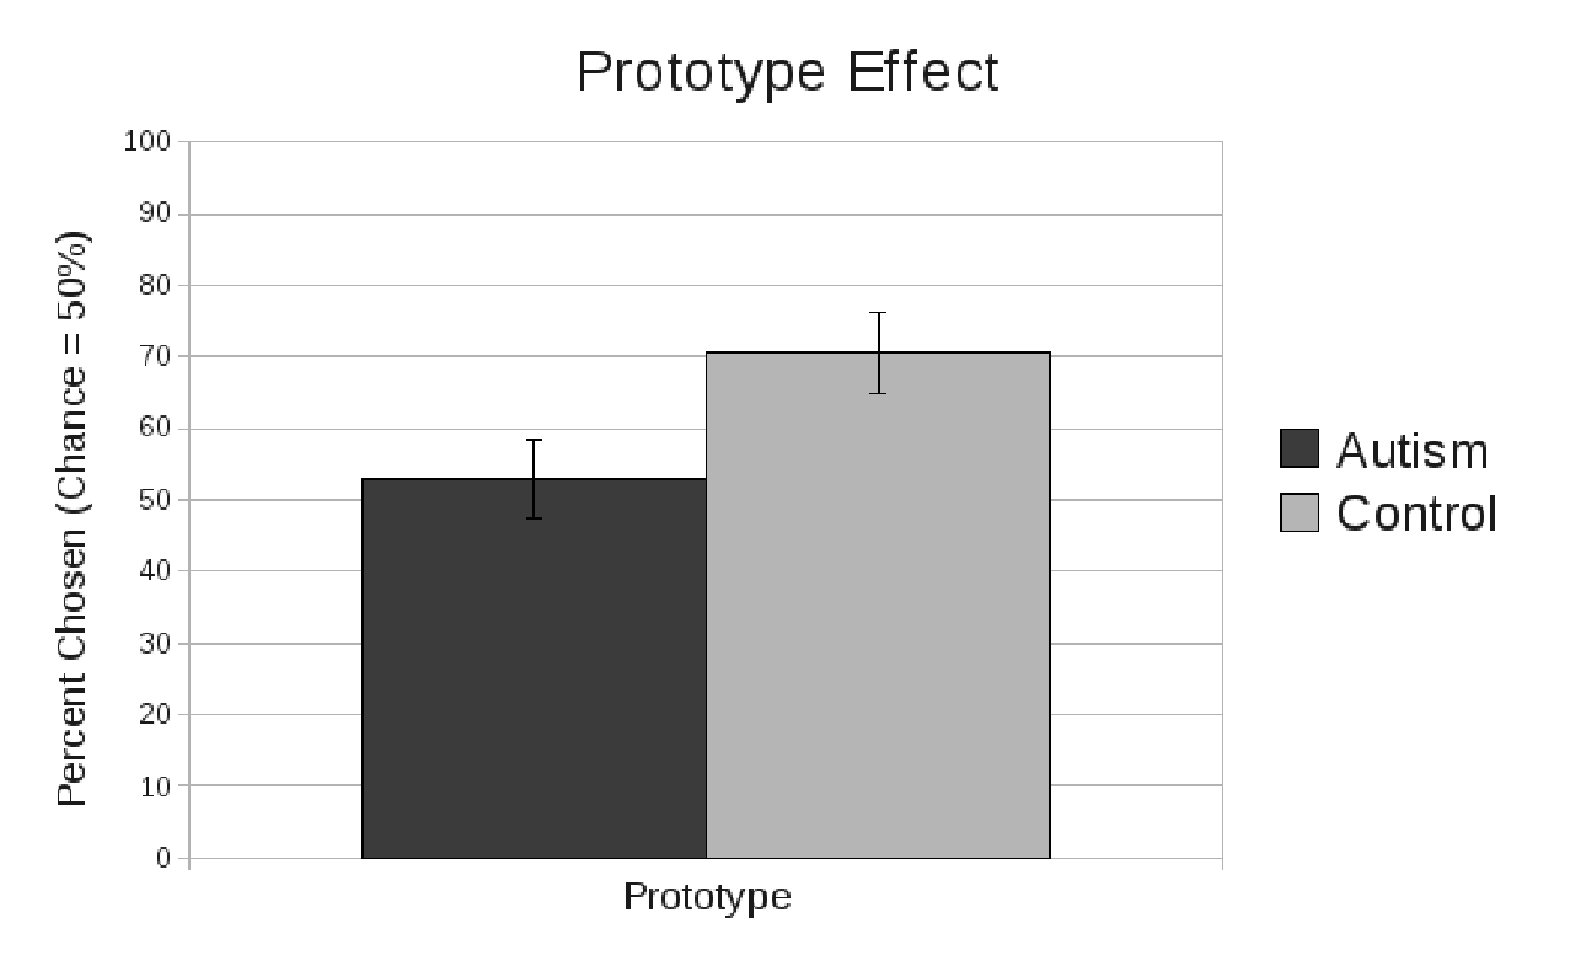
\includegraphics[width=100mm]{graphs/alcove_results.eps}
\end{center}
\caption{ALCOVE Model Results.  The measure on the y-axis is the percentage of times that the prototypical animal was chosen by the model over the non-prototype choices.  In the control network, the prototype was chosen 70.52\% of the time on average, demonstrating a strong prototype effect and matching the human subject experiment results.  However, the model of autistic performance chose the prototype on average only 52.91\% of the time over the non-prototype stimuli.  Statistical analysis reveal that the control network chose the prototype at a rate significantly greater than chance ($p < .0001$) while the ASD network was not statistically distinguishable from chance ($p > .30$).}
\label{alcove-results}
\end{figure} 

\section{Summary}

The results presented here support the feasibility of explaining the categorization performance of people with autism in terms of my hypothesized deficit, dysfunctional interactions between the mid-bran DA system and PFC.  In this chapter, the widely used ALCOVE model was modified in order to simulate how inflexible updating of the contents of PFC would manifest within ALCOVE's framework. Restricting the ability of ALCOVE's global attentional mechanism to spread its influence evenly over all features of a stimulus results in a lack of prototype preference in the network.  This manipulation is functionally the same as the deficit that has been posited in previous chapters to explain distinct behavioral patterns in people with ASD including executive dysfunction, overselective behavior, implicit learning deficits, and problems disambiguating the contextual information during sentence processing.      

